\iffalse
\documentclass[journal,12pt,twocolumn]{IEEEtran}
\usepackage{cite}
\usepackage{amsmath,amssymb,amsfonts,amsthm}
\usepackage{algorithmic}
\usepackage{graphicx}
\usepackage{textcomp}
\usepackage{xcolor}
\usepackage{txfonts}
\usepackage{listings}
\usepackage{enumitem}
\usepackage{mathtools}
\usepackage{float}
\usepackage{gensymb}
\usepackage{comment}
\usepackage[breaklinks=true]{hyperref}
\usepackage{tkz-euclide} 
\usepackage{listings}
\usepackage{gvv}                                        
\def\inputGnumericTable{}                                 
\usepackage[latin1]{inputenc}                                
\usepackage{color}                                            
\usepackage{array}                                            
\usepackage{longtable}                                       
\usepackage{calc}            
\usepackage{multirow}                                         
\usepackage{hhline}                                           
\usepackage{ifthen}                                           
\usepackage{lscape}
\usepackage{amsmath}
\newtheorem{theorem}{Theorem}[section]
\newtheorem{problem}{Problem}
\newtheorem{proposition}{Proposition}[section]
\newtheorem{lemma}{Lemma}[section]
\newtheorem{corollary}[theorem]{Corollary}
\newtheorem{example}{Example}[section]
\newtheorem{definition}[problem]{Definition}
\newcommand{\BEQA}{\begin{eqnarray}}
\newcommand{\EEQA}{\end{eqnarray}}
\newcommand{\define}{\stackrel{\triangle}{=}}
\theoremstyle{remark}
\newtheorem{rem}{Remark}

\begin{document}

\bibliographystyle{IEEEtran}
\vspace{3cm}

\title{NCERT Discrete - 10.5.2.1}
\author{EE23BTECH11037 - M Esha$^{*}$}

\maketitle
\newpage
\bigskip

\renewcommand{\thefigure}{\theenumi}
\renewcommand{\thetable}{\theenumi}

\vspace{3cm}
\textbf{Question 10.5.2.1:} 

 Fill in the blanks in the following table given that $a$ is the first term, $d$ is the common difference, and $a_n$ is the $n$th term of the AP.

\begin{table}[h!]
  \centering
  \begin{tabular}{c@{\hspace{1cm}}c@{\hspace{1cm}}c@{\hspace{1cm}}c}
    \hline
    $a$ & $d$ & $n$ & $a_n$ \\
    \hline
    7 & 3 & 8 & ... \\
    -18 & ... & 10 & 0 \\
    ... & -3 & 18 & -5 \\
    -18.9 & 2.5 & ... & 3.6 \\
    3.5 & 0 & 105 & ... \\
    \hline
  \end{tabular}

   \label{tab:ESTable1}
\end{table}
\solution
\fi
for A.P,
\begin{align}
    x_i(n) = \sbrak{x_i(0) + nd_i} u(n)
    \label{eq:ES1}
\end{align}
\begin{enumerate}
\item From \eqref{eq:ES1} :
\begin{align}
x_1(n) &= \sbrak{7+3n}u(n)\\
x_1(7) &= 28\\
X_1(z) &= \frac{7 - 4z^{-1}}{(1 - z^{-1})^2} \quad |z| \neq 1
\end{align}
\item From \eqref{eq:ES1}:
\begin{align}
x_2(n) &= \sbrak{-18 + d_2n}u(n)\\
x_2(9) &= 0\\
d_2 &= 2\\
X_2(z) &= \frac{-18 + 20z^{-1}}{(1 - z^{-1})^2}
 \quad |z| \neq 1
\end{align}
\item From \eqref{eq:ES1} :
\begin{align}
x_3(n) &= \sbrak{x_3(0)-3n}u(n)\\
x_3(17) &= -5\\
x_3(0) &= 49\\
X_3(z) &= \frac{49 - 52z^{-1}}{(1 - z^{-1})^2}
 \quad |z| \neq 1
\end{align}
\item From \eqref{eq:ES1} :
\begin{align}
x_4(n) &= \sbrak{18.9+2.5n}u(n)\\
x_4(n) &= 3.6\\
n_4    &= 9\\
X_4(z) &= \frac{18.9 - 16.4z^{-1}}{(1 - z^{-1})^2}
 \quad |z| \neq 1
\end{align}
\item From \eqref{eq:ES1}  :
\begin{align}
x_5(n) &= \sbrak{3.5}u(n)\\
x_5(104) &= 3.5\\
X_5(z) &= \frac{3.5}{1-z^{-1}} \quad |z| \neq 1
\end{align}
\begin{figure}[h!]
    \centering
    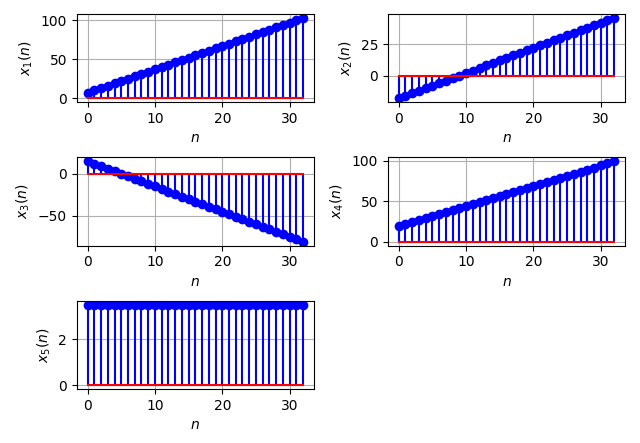
\includegraphics[width=\columnwidth]{ncert-maths/10/5/2/1/figs/10.png}
    \caption{stem plots }
    \label{fig:ESFIG1}
\end{figure}
\end{enumerate}

%\end{document}

